\documentclass{beamer}
\usetheme{Szeged}
\usecolortheme{beaver}

\usepackage{minted}
\usemintedstyle{pastie}

\usepackage{graphicx}
\usepackage{hyperref}
\hypersetup{
    colorlinks=true,
    linkcolor=blue,
    filecolor=magenta,      
    urlcolor=cyan,
}

\title{Discussion 01}
\subtitle{Welcome to 3110!}
\author{Kenneth Fang (kwf37), Newton Ni (cn279)}
\date{Jan. 28, 2019}

\begin{document}

    \begin{frame}
        \titlepage{}
    \end{frame}
    
    \begin{frame}{Logistics}
    \begin{itemize}
        \item This is Discussion 213, MoWe 10:10AM-11:00AM
        \item Discussions will generally consist of short review followed by exercise problems
        \item Attendance will be taken using One-Minute-Memos (OMMs) starting \textbf{Wednesday}
        \item Exercises and slides will be posted on this GitHub Repo: \url{https://github.com/nwtnni/discussion-sp19}
    \end{itemize}
    \end{frame}
    
    
    \begin{frame}{Kenneth Fang}
    \begin{columns}
        \begin{column}{0.48\textwidth}
            \begin{itemize}
                \item Junior in ECE/CS
                \item Interested in Programming Languages, Computer Architecture, Analog and Digital Integrated Circuit Design
                \item Ask me about ECE, Theatre Lighting, Frisbee, Video Games
            \end{itemize}
        \end{column}
        \begin{column}{0.48\textwidth}
            \begin{figure}
                \centering
                
\includegraphics[scale=0.8]{kwf37.jpg}
                \caption{A Spooky Dude}
            \end{figure}
        \end{column}
    \end{columns}
    \end{frame}
    
    \begin{frame}{Newton Ni}
        \begin{columns}
            \begin{column}{0.48\textwidth}
                \begin{figure}
                    \centering
                    
\includegraphics[scale = 0.20]{cn279.jpg}
                    \caption{A Physics Dropout}
                \end{figure}
            \end{column}
            \begin{column}{0.48\textwidth}
                \begin{itemize}
                    \item Senior in CS
                    \item Interested in Programming Languages, Compilers, Systems
                    \item Ask me about Rust, Rocket League, Vim
                \end{itemize}
            \end{column}
        \end{columns}
    \end{frame}
    
    \begin{frame}{Introductions}
        Please tell us your $\ldots$
        \begin{itemize}
            \item Name
            \item Favorite Household Appliance
            \item Ex: My name is Kenneth and I like toasters.
        \end{itemize}
    \end{frame}
    
    \begin{frame}{Questions about the Course?}
        \begin{figure}
            \centering
            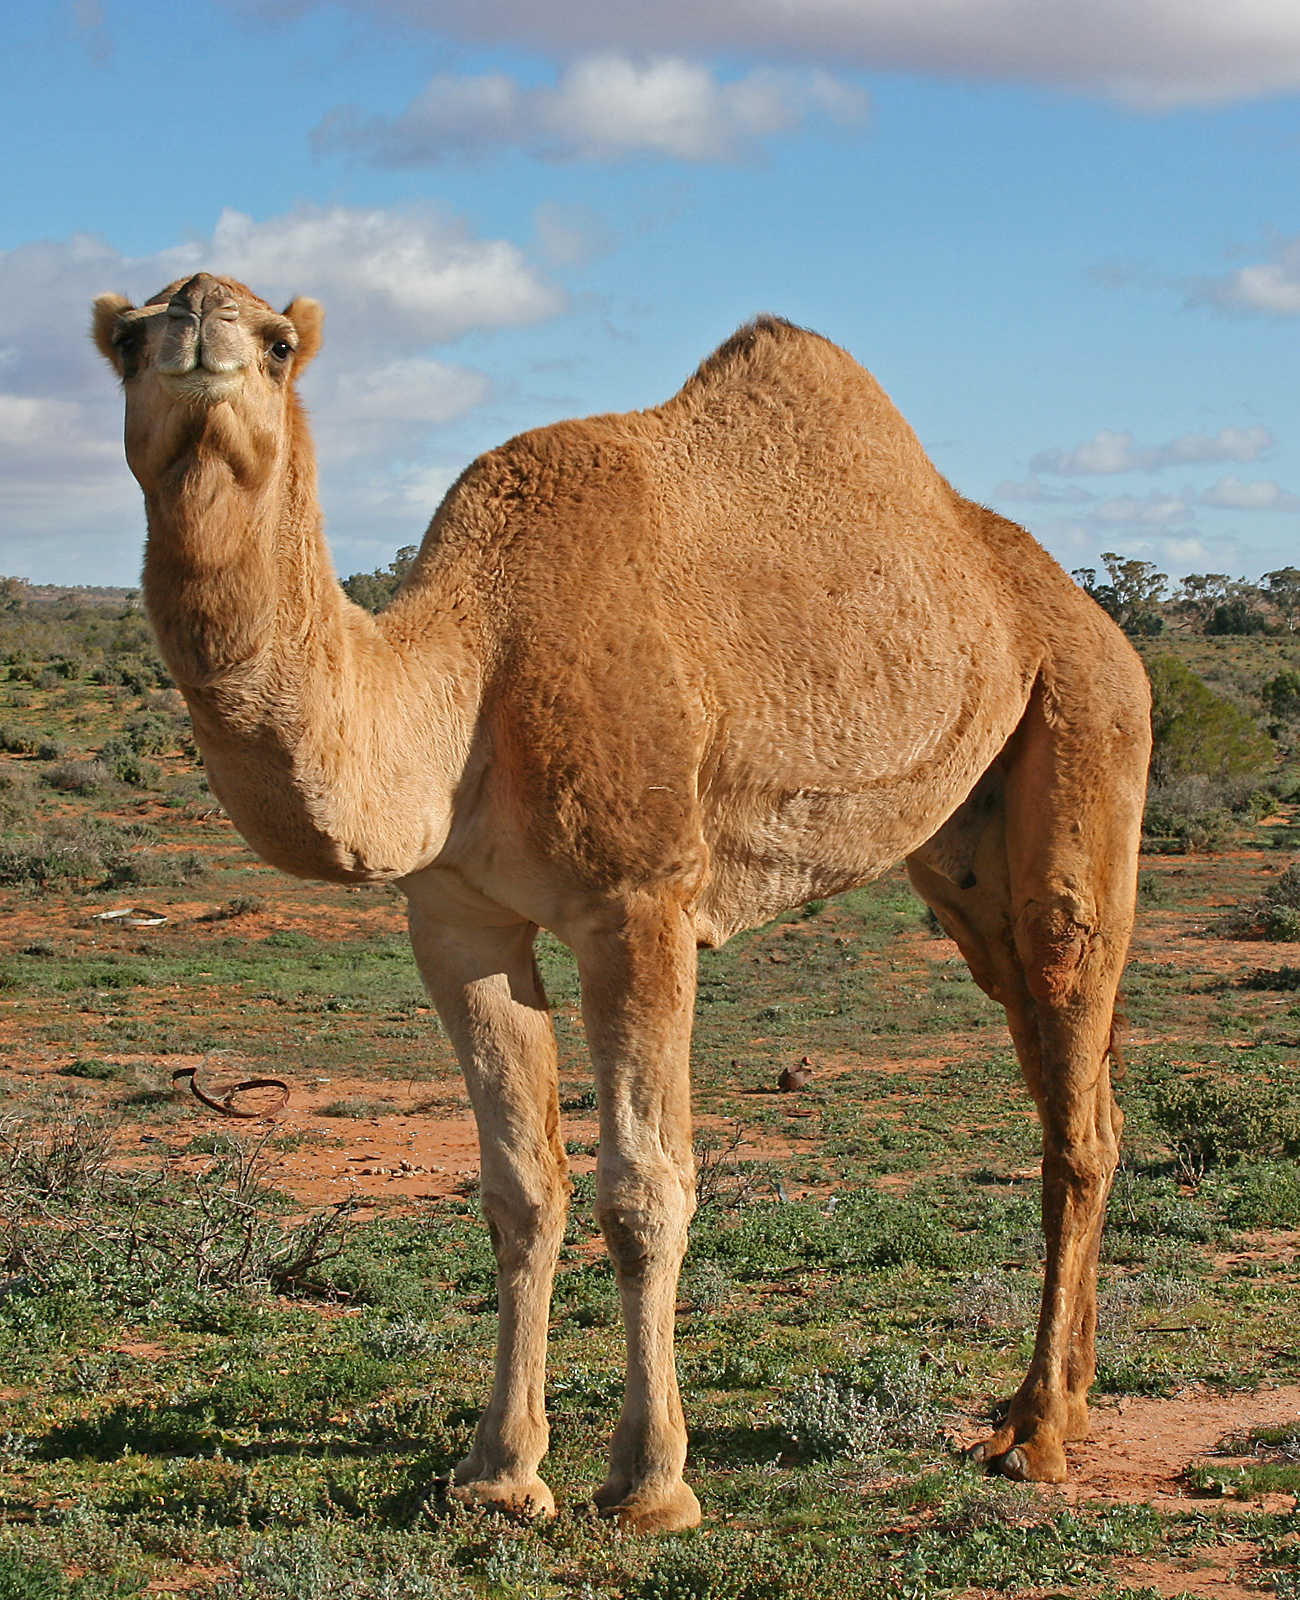
\includegraphics[scale = 0.1]{camel.jpg}
            \caption{What am I doing here?}
        \end{figure}
    \end{frame}
    
    \begin{frame}{Let Expressions}
        \begin{itemize}
            \item Let expressions have the following form:
            \item \mint{ocaml}{let x = e1 in e2}
            \item Where \texttt{x} is an identifier and \texttt{e1}, \texttt{e2} are expressions
        \end{itemize}
    \end{frame}
    
    \begin{frame}{Let Expressions: Dynamic Semantics}
        \begin{itemize}
            \item How to \textbf{evaluate} expressions
            \item Here are the dynamic semantics for let expressions:
            \begin{enumerate}
                \item Evaluate e1 to a value, we'll call it v1
                \item Look for the identifier x and substitute x for v1 everywhere in e2. This gives us a new expression e2'
                \item Evaluate e2' to a value v2. This is the result of evaluating the let expression.
            \end{enumerate}
        \end{itemize}
    \end{frame}
    
    \begin{frame}{Let Expressions: Dynamic Semantics}
        \begin{itemize}
            \item \mint{ocaml}{let z = 0 + 1 in z + 41}
            \item \mint{ocaml}{let z = 1 in z + 41}
            \item \mint{ocaml}{1 + 41}
            \item \mint{ocaml}{42}
        \end{itemize} 
    \end{frame}
    
    \begin{frame}{Let Expressions: Dynamic Semantics}
        \begin{itemize}
            \item \mint{ocaml}{let y = 25 in let z = y * 3 in z - y}
            \item \mint{ocaml}{let z = y * 3 in z - y }
            \item \mint{ocaml}{let z = 25 * 3 in z - 25}
            \item \mint{ocaml}{let z = 75 in z - 25}
            \item \mint{ocaml}{z - 25}
            \item \mint{ocaml}{75 - 25}
            \item \mint{ocaml}{50}
        \end{itemize} 
    \end{frame}
    
    \begin{frame}{Let Expressions: Static Semantics}
        \begin{itemize}
            \item How to \textbf{type-check} expressions
            \item Here are the static semantics for let expressions:
            \begin{enumerate}
                \item If \texttt{e1} has type \texttt{t1}
                \item If \texttt{e2} has type \texttt{t2} given that \texttt{x} has type \texttt{t1}
                \item Then the let expression has type \texttt{t2}
            \end{enumerate}
        \end{itemize}    
    \end{frame}
    
    \begin{frame}{Recitation Questions}
    \end{frame}

\end{document}

